\chapter{REAL-TIME PARTICLE SYSTEMS LIBRARY}\label{RTPSchapter}

% Introduction
%\section{Introduction}
The Real-Time Particle Systems (RTPS) library was designed and developed by Ian Johnson\cite{ianPaper}. The RTPS library is able to simulate various particle systems including Smooth Particle Hydrodynamics (SPH) and Flocking (Boids) systems. The \texttt{FLOCK} system was created by us.

This chapter introduces the RTPS framework. The description of the RTPS library follows the structure of the RTPS implementation showed in Figure~\ref{RTPSdiagram}. At the end of the Chapter a detailed description of the extended implementation developed for the \texttt{FLOCK} system is given. 

% RTPS diagram
\begin{figure}[htbp]
\begin{center}
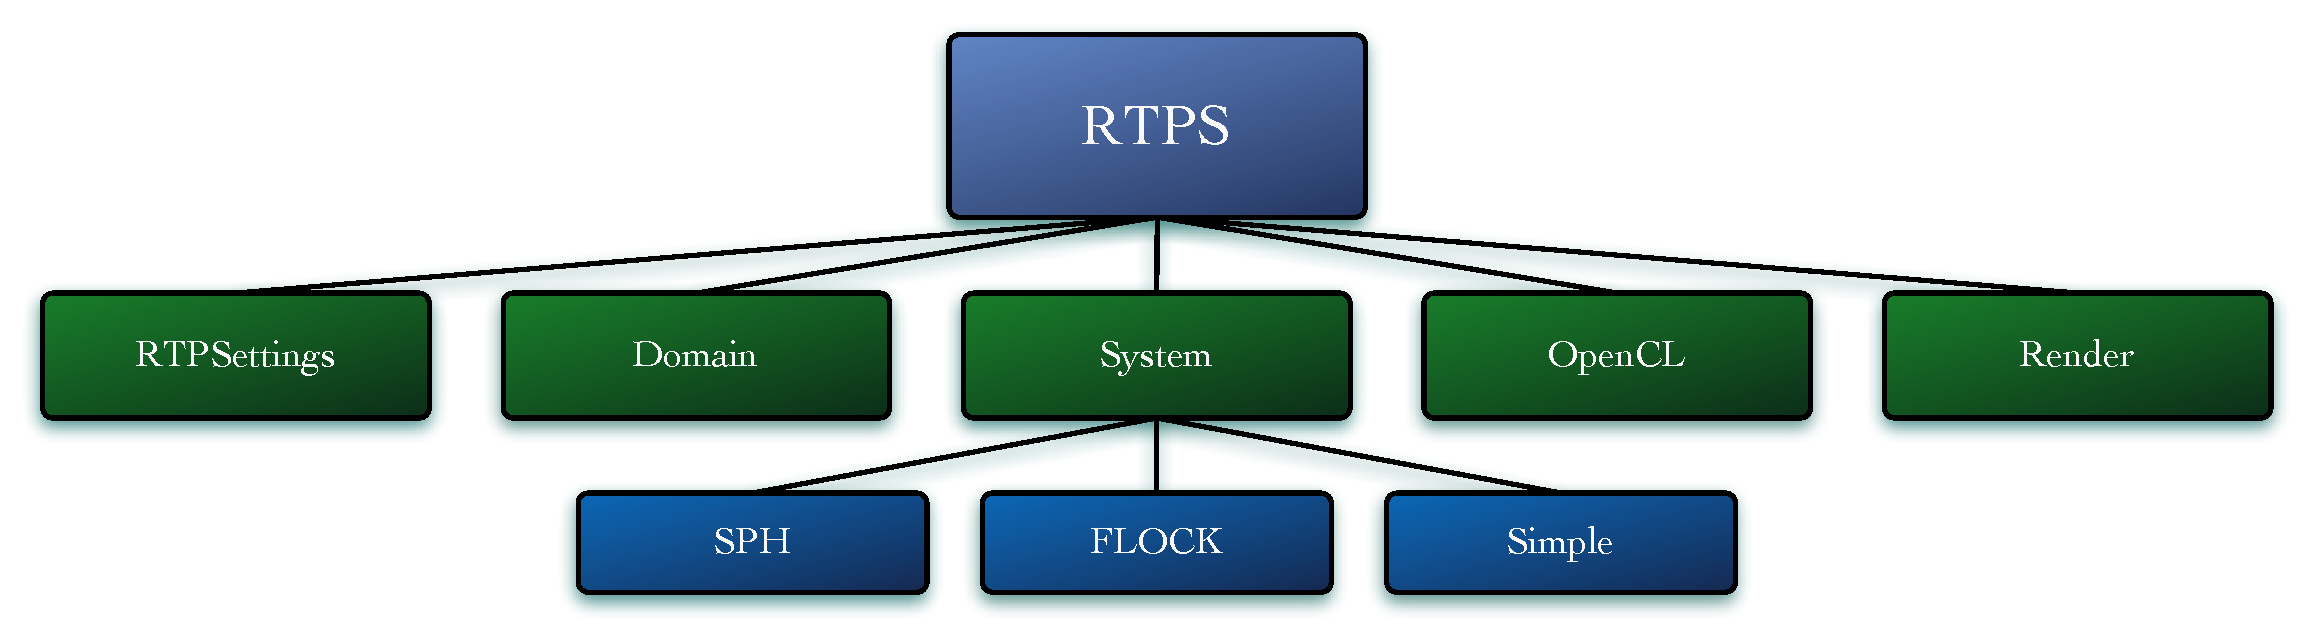
\includegraphics[scale=0.30]{figures/RTPSdiagramMyrna.pdf}
\caption{RTPS hierarchy diagram: depicts the structure of the RTPS library}
\label{RTPSdiagram}
\end{center}
\end{figure}

% RTPS
\section{RTPS}\label{rtpssection}
\texttt{RTPS.h} is the main class of the RTPS library. An \texttt{RTPS} object is particle system, this system might be initialized with given a set of settings. The settings are discussed in Section~\ref{rtpsettings}. 

As seen in Figure~\ref{RTPSdiagram}, \texttt{RTPS} is the head of the library. Only two methods are defined in the \texttt{RTPS} class: \texttt{update()} and \texttt{render()}. \texttt{update()} computes the positions of the particles at each frame, and \texttt{render()} is in charge of rendering the particles. These methods are implemented individually by each of the systems available in the RTPS library. The following code shows the \texttt{RTPS} constructor used when creating the \texttt{FLOCK} system.

%\texttt{RTPS} has various instance variables: a \texttt{CL} object which is used to manage the \textit{OpenCL} functionality,  an \texttt{RTPSettings} object to manage the settings of the system and a \texttt{System} object which stores the type of particle system that has been created. 
% RTPS constructor

\begin{cppcode}{0}
RTPS::RTPS(RTPSettings *s, CL* _cli) 
{
	cli = _cli;
 	cl_managed = false;
	settings = s;
	Init();
}
\end{cppcode}

The \texttt{Init()} method called inside the constructor would creates the respective particle system, i.e. \texttt{SPH} or \texttt{FLOCK}, depending on the settings.

% RTPSettings
\section{RTPS Settings}\label{rtpsettings}
\texttt{RTPSettings} is the class that stores all the settings of the particle systems. This class defines the set of systems available in RTPS. The settings are defined depending on the systems. The three systems currently available are: SPH, FLOCK and Simple. The constructor used to create the RTPS  settings is presented bellow. \texttt{Systype} is an enumeration that has the names of the systems stated above.

%The location of this class is at \texttt{rtpslib/RTPSettings.h}. It has the following instance variables defined: the maximum number of particles, the time step, and a \texttt{Domain} object. Also, there is an enumeration variable \texttt{SysType} that defines the names of the three available particle systems. Some of the rendering settings are set and get in this class. Here is the \texttt{RTPSettings} constructor that we use for the \texttt{FLOCK} system.

% RTPSettings constructor
\begin{cppcode}{0}
RTPSettings::RTPSettings(SysType system, int max_particles, float dt, Domain* grid)
{
	changed = false;
	this->system = system;
	this->max_particles = nlpo2(max_particles);
	this->dt = dt;
	this->grid = grid;
}
\end{cppcode}

%The parameters for this constructor are the type of system, the maximum number of particles, the time step and the grid domain. 

As an OpenCL requirement, the maximum number of particles has to be a power of two. That is why the variable \texttt{max\_particles} is processed through the function \texttt{nlpo2}, which takes care of that.

% Domain
\section{Domain}
The \texttt{Domain} class defines the grid in which the simulation is being computed. This class also stores all the different grid parameters that are needed through out the computation process. The \texttt{IV} class is defined in the same folder than the \texttt{Domain} class. The \texttt{IV} class defines and implements the methods that initialize the positions of the particles. Various geometric shapes are available: rectangles, spheres, and discs. The \texttt{UniformGrid} class is also defined in the same folder than the \texttt{Domain} class. \texttt{UniformGrid} class is used in the nearest neighbor search.

% Render
\section{Render}
Most of the code developed to do the render for the RTPS library was developed by Andrew Young\cite{andrewBlog}. There are different types of rendering defined in the RTPS library. \texttt{Render} type renders the particles as Points. \texttt{SpriteRender} use a 2D image and mapped into a sphere and render the particles as those spheres. \texttt{SSFRender} is more used for the SPH system. \texttt{Sphere3DRender} renders the boids as 3D spheres.  

% System
\section{System}
Each of the particle systems in the RTPS library inherits the \texttt{System} class which contains virtual functions that are shared by the systems. These functions are related to the rendering,  the domain, and to other shared classes. There are three systems that extends the \texttt{System} class. Those systems are: \texttt{SPH}, \texttt{FLOCK}, and \texttt{Simple}. The \texttt{SPH} system is going to be briefly discussed in Section~\ref{sphsection}. The \texttt{FLOCK} system would be described in detail in Section~\ref{flocksection}. The \texttt{Simple} system was created for testing and debugging the \texttt{SPH} system.

% Common
\section{Common}\label{commonsection}
The RTPS library has shared classes that are used for all systems. These classes include the implementation of a hose. The hose is used to spray particles into the system. The other common classes include the classes for the nearest neighbor search. The next section explains how the nearest neighbor search is done. 

\subsection{Nearest Neighbor Search}
The approach taken to do the implemented nearest neighbor search is divided in two phases: \textit{preparation} and \textit{lookup}. The following following steps explains how the \textit{preparation} phase is done.

\begin{enumerate}
\item{\textbf{Hash}: creates a hash value by overlaying a uniform grid at the system's domain, and calculating a index value from the 3D cell index}
\item{\textbf{Sort}: sorts the hash array by the hash values, an array with the initial indices of the particles is also sorted according the hash values}
\item{\textbf{Permute}:  permutes the arrays of positions, velocities, and color according to the sorted index array}
\item{\textbf{Cell indices}: updates two arrays: \texttt{cell\_indices\_start} and \texttt{cell\_indices\_end} which keep track of which cell are populated with particles, \texttt{cell\_indices\_start} stores the index of the first particle in each cell, when there is no particle an index of $-1$ is assigned; the \texttt{cell\_indices\_end} arrays stores the index of the last particle in that cell}
\end{enumerate}

After the preparation is done arrays are ready to be access it, this meaning that are ready for the neighbor searching. The access of  the arrays is made during the lookup phase of the nearest neighbor search. This phase consists of calling the following three functions:

\begin{enumerate}
\item{\textbf{IterateParticleInNearbyCells}: loops over the 26 cells surrounding the cell of the particle in question, this function calls \texttt{IterateParticlesInCells} for each cell }
\item{\textbf{IterateParticlesInCells}: loops over the particles from the start index to the end index of that cell and calls \texttt{ForNeighbor} for each particle}
\item{\textbf{ForNeighbor}: access the particle in question and the neighboring particle}
\end{enumerate}

Having the particle information and the neighbor particle information, then we do calculations between them. The three main steering behaviors of flocking use the nearest neighbor search to compute the respective rule in the local neighborhood of each boid.

% SPH
\section{SPH}\label{sphsection}
The \texttt{SPH} system is the main system of the RTPS library. It was developed and it is currently maintained by Ian Johnson\cite{ianBlog}\cite{ianPaper}. This system uses the SPH formulation to compute the different forces between particles.

The only difference between the \texttt{FLOCK} system and the \texttt{SPH} system is that \texttt{SPH} calculates forces while \texttt{FLOCK} calculates velocities. The algorithm followed is very very similar. The SPH formulation is used to compute forces while the boids only need to compute their steering behaviors to compute the velocities. At the end both systems integrate over time to update the positions of the particles.

For a more detailed information about the \texttt{SPH} system implemented in the RTPS library, please refer to Ian Johnson Master Thesis\cite{ianThesis}.

% FLOCK
\section{FLOCK}\label{flocksection}
The \texttt{FLOCK} system is the system of our concern. The \texttt{SPH} system was used as a guide to create the \texttt{FLOCK} system. Both of these systems are extensions of  the \texttt{System} class. The main class of the \texttt{FLOCK} system is also called \texttt{FLOCK}. The settings of the \texttt{FLOCK} system are stored in the \texttt{FLOCKSettings} class. 

The three main steering behaviors of flocking in addition to the goal and avoid behaviors were implemented. Figure~\ref{flockdiagram} shows the hierarchy of the \texttt{FLOCK} system. The \texttt{FLOCK} and \texttt{FLOCKSettings} are discussed later in this Section. The common classes were already discussed in Section~\ref{commonsection}. The \texttt{Rules} and \texttt{EulerIntegration} classes are discussed at the end of this Section.

% FLOCK diagram
\begin{figure}[htbp]
\begin{center}
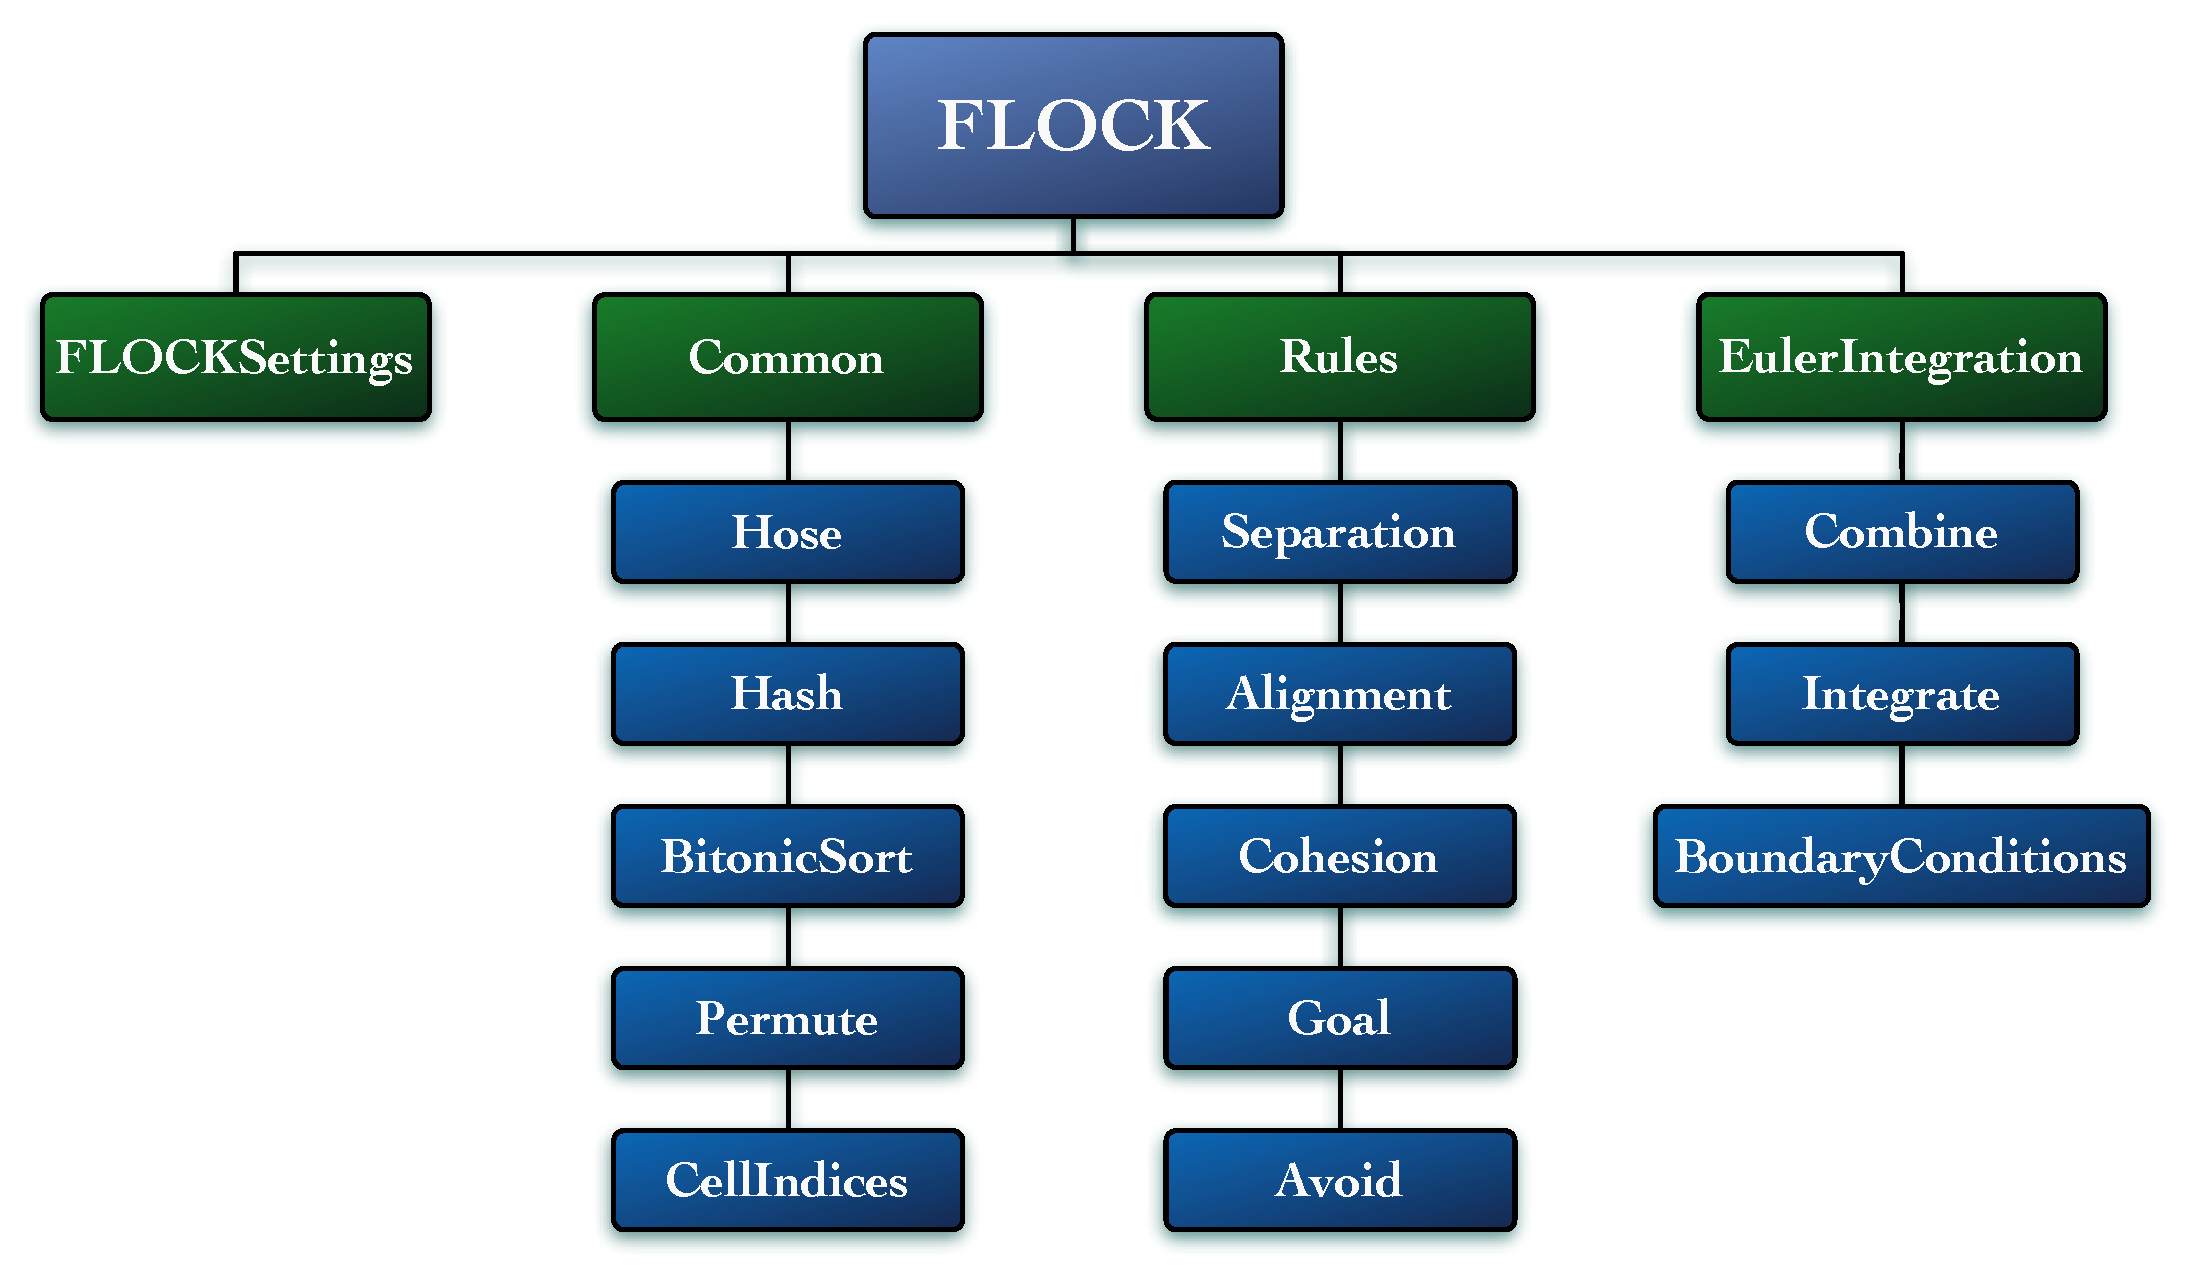
\includegraphics[scale=0.3]{figures/FLOCKdiagramMyrna.pdf}
\caption{FLOCK hierarchy diagram: depicts the hierarchy of the classes developed for the FLOCK system}
\label{flockdiagram}
\end{center}
\end{figure}


% FLOCK class
\subsection{FLOCK class}
As mentioned before the \texttt{FLOCK} class is the main class of our system. The header file of this class defines the prototypes of the functions that are used to insert particles into our system. Also, all the vectors and buffers used to store the information of of the particles in the CPU and GPU are declared in the header file. The following code shows some of the main step in the constructor of our class.

\begin{cppcode}{0}
FLOCK::FLOCK(RTPS *psfr, int n)
 {
 	//store the particle system framework
 	ps = psfr;
	settings = ps->settings;
	grid = settings->grid;
	max_num = n;
	
	// initial number of particles
	num = 0;
 	
	...
 
 	// calculate and update the parameters
	calculate();
	updateFLOCKP();

	...

	//set up the grid
	setupDomain();
	
	//setup the sorted and unsorted arrays
	prepareSorted();
 	 
	 ...
		
	// create the renderer object depending on the render type		
	setRenderer(); 
}
\end{cppcode}

At the beginning some of the instance variables of \texttt{FLOCK} are set to the respective values obtained from the arguments. 

Then, the initial settings of the system are calculated and updated. The settings of \texttt{FLOCK} are stored in a struct called \texttt{FLOCKParameters}. When executing \texttt{calculate()}, the parameters are set to the default values. Then, the \texttt{updateFLOCKP()} updates the parameters to the settings set by the user. 

Next, is the setup of the domain. During the setup of the domain, the grid parameters are initialized.

The function \texttt{prepareSorted()} initializes the different vectors and buffers that were created for our system i.e \texttt{velocities}, \texttt{flockmates}, etc. This function also creates the VBOs. VBOs stands for Vertex Buffer Objects and these buffer objects are used to store vertex data that its aim to be used for rendering purposes\cite{vbo}. Then, the positions and color vectors are copied to the respective VBOs. If using the GPU the different \texttt{Buffer} objects are initialized with their respective CPU arrays. The \texttt{FLOCK} parameters are also copied to the GPU. 

The \texttt{setRenderer()} function creates the \texttt{renderer} object depending on which render type was set at the \texttt{RTPSettings}.

\subsubsection{Particles insertion}
The system has being created and now the question arise in \textit{how do the particles are inserted into the system?} There are a few functions defined in the \texttt{FLOCK} that do that task. These functions are \texttt{addBox} , \texttt{addBall}, and \texttt{addHose}. First, these functions initialize the positions of the particles then the positions of the particles are send to the GPU or CPU to be rendered. 

\subsubsection{Update}
As mentioned in Section~\ref{rtpssection} each of the systems would implement the methods \texttt{update()} and \texttt{render()}, respectively. In \texttt{FLOCK} the \texttt{update()} function updates the positions of the boids at each frame. If using the CPU, the \texttt{updateCPU()} function is called. \texttt{updateCPU()} calls the functions \texttt{cpuRules()} and \texttt{cpuEulerIntegration()} which compute the rules sequentially in the CPU and integrates to retrieve the new positions of the boids. The CPU code was developed for testing and debugging purposes only. On the other hand, if using the GPU to do the calculations, the \texttt{updateGPU()} function is called. \texttt{updateGPU()} calls the OpenCL kernels that do the nearest neighbor search, then computes the flocking rules and finally integrates to get the new positions. These kernels are described in more detail in Section~\ref{rulesclass}.


% FLOCKSettings class
\subsection{FLOCKSettings class}
In order to run a simulation, the settings of the system need to be set. The flocking specific settings are defined in the class called \texttt{FLOCKSettings}. The \texttt{FLOCKParameters} struct stores all these settings. 

The \texttt{FLOCKParameters} struct include variables as the simulation scale, the searching radius, the maximum speed of the boids and the weights of each of the steering behaviors. In the implementation file of the \texttt{FLOCKSettings} class are the functions \texttt{calculate()} and \texttt{updateFLOCKP()}.

% Rules class
\subsection{Rules class}\label{rulesclass}
The \texttt{Rules} class computes the different steering behaviors that were implemented to simulate the flocking behavior. The steering behaviors or \textit{rules} are implemented in both CPU and GPU code. Each of the rules implemented for the GPU execution is defined in the \texttt{rules} kernel. The following code is the \texttt{Rules.h} file which defines the \texttt{Rules} class.

\begin{cppcode}{0}
#ifndef RTPS_RULES_H_INCLUDED
#define RTPS_RULES_H_INCLUDED

#include <CLL.h>
 #include <Buffer.h>

namespace rtps
 {
	class Rules
	{
		public:
			// constructors
			Rules() { cli = NULL; timer = NULL; };
			Rules(std::string path, CL* cli, EB::Timer* timer);
			
			// execution of kernels
			void execute( /* arguments */ );
			
		private:
			// OpenCL
			CL* cli;
			
			// kernels
			Kernel k_rules;
			
			// timer
			EB::Timer* timer;
	};
}
#endif
\end{cppcode}

The implementation of the function that executes the kernel is in \texttt{Rules.cpp}. First, the kernel is initialized in the constructor of the \texttt{Rules} class, then inside the implementation of the \texttt{execute()}, the arguments of the kernel are set. In this file \texttt{Rules.cpp} is where the \texttt{cpuRules()} function is implemented. Part of the \texttt{Rules.cpp} file is show next.

\begin{cppcode}{0}
#include<FLOCK.h>
#include<math.h>

namespace rtps
{
	// Rules constructor
	Rules::Rules(std::string wpath, CL* cli_, EB::Timer* timer_)
	{
		...
		try
		{
			path = wpath + "/rules.cl";
			k_rules = Kernel(cli, path, "rules");
		}
		....
	}

	void Rules::execute( /* arguments */ )
	{
		// set the arguments for the kernel
		int iarg = 0;
		k_rules.setArg(iarg++, pos_s.getDevicePtr());
		k_rules.setArg(iarg++, vel_s.getDevicePtr());
		...
	}
	...
	
	void FLOCK::cpuRules()
	{
		...
	}
}
\end{cppcode}

The implementation of the kernel was done in a separate folder. This would help us to better distinguish between the C++ and the OpenCL files. The kernel defined in \texttt{Rules} is called \texttt{rules}. Each rule was implemented in an individual file that is included where the respective rule is called. Those files are \texttt{rule\_separation}, \texttt{rule\_alignment}, \texttt{rule\_cohesion}, \texttt{rule\_goal}, and \texttt{rule\_avoid}. The \texttt{rules} kernel implements the Algorithm~\ref{flockingAlgorithm}.

%, and \texttt{rule\_leaderfollowing}.

%\texttt{\textbf{flockmates}} looks for the neighbors and determines which ones are within the searching radius, and count them. Also, it counts how many neighbors are within the minimum separation distance of each boid. At the end, the vector \texttt{flockmates} which was allocated in the GPU is updated with the values obtained.

%\texttt{\textbf{rule\_separation}} is computed using the neighbors that are within the minimum separation distance\footnote{for more details on how the rule is computed see the formulation of Separation in Section~\ref{separationsection}}. The behavior is accumulated in a vector. After the neighbors within the minimum distance are processed, the behavior vector is averaged over the number of flockmates found within the minimum separation distance, then the vector is normalized. Finally, the value of the vector \texttt{separation} are copied to the vector allocated in the GPU.

%\texttt{\textbf{rule\_alignment}} determines which neighbors are within a prescribed radius, the velocities of those neighbors are accumulated. Then, the average is taken using the number of flockmates following by a subtraction of the average velocity and the boids velocity. At the end the vector obtained is used to update the respective vector in the GPU. 

%\texttt{\textbf{rule\_cohesion}} is analogous to the alignment rule, the only difference is that positions are used instead of velocities.

%\texttt{\textbf{rule\_leaderfollowing}} \textcolor{red}{*** TODO: still need to develop the leader behavior, then I would write the description of this kernel ***}

%This would finish the description of the \texttt{Rules} class. The next step is to integrate over time to get the new position of the boid.

% Euler Integration class
\subsection{EulerIntegration class}
%A discussion on how to get the different steering behaviors vectors have been done. 
This section describes briefly how to combine the vectors that stores the behaviors in order to get one single vector to update the positions. A class called \texttt{EulerIntegration} was developed in order to get the new positions. The {EulerIntegration.h} class is show bellow.

\begin{cppcode}{0}
#ifndef RTPS_EULER_INTEGRATION_H_
#define RTPS_EULER_INTEGRATION_H_

#include <CLL.h>
#include <Buffer.h>

namespace rtps
{
	class EulerIntegration
	{
		public:
			EulerIntegration() { cli = NULL; timer = NULL; };
	 		EulerIntegration(std::string path, CL* cli, EB::Timer* timer);
			void execute( /* arguments */ );

		private:
			CL* cli;
			Kernel k_euler_integration;
			EB::Timer* timer;
	};
}
#endif
\end{cppcode}

The \texttt{EulerIntegration} class structure is similar to the \texttt{Rules} class structure. The \texttt{EulerIntegration.cpp} initializes the kernel and implements the \texttt{execute} function which sets the arguments of the kernels and executes it. It also has the implementation of the \texttt{cpuEulerIntegration()} function. The name of the OpenCL kernel developed for the GPU is \texttt{euler\_integration}, it is also located in the same folder along with the \texttt{rules} kernel.

\texttt{\textbf{euler\_integration}} starts by getting the respective steering vectors from the GPU, and also getting the weights of each of the rules. The weights are gotten from the flocking parameters object. Then, the velocity vectors for each of the rules are computed and combined to get the final velocity vector.

\begin{cppcode}{0}
// RULE 1. SEPARATION
vel_sep = separation * w_sep;
   
// RULE 2. ALIGNMENT
vel_aln = alignment * w_aln;

// RULE 3. COHESION
vel_coh = cohesion * w_coh;

// RULE 4. GOAL
vel_goal = goal * w_goal;

// RULE 5. AVOID
vel_avoid = avoid * w_avoid;

// GLOBAL ACCELERATION
vel = vi + vel_sep + vel_aln + vel_coh + vel_goal + vel_avoid;
\end{cppcode}

After obtaining the global velocity vector, this vector is constrained to the maximum speed. 

An optional circular velocity field that modifies the velocity can be added to the boids' velocity. The constant that weights how strong this velocity field is, is stored in the flocking parameters.

\begin{cppcode}{0}
// OPTIONAL CIRCULAR VELOCITY FIELD
float4 v = (float4)(-3*pi.z, 0.f , pi.x, 0.f);
v *= flockp->circular_vel_const;

// SET THE NEW VELOCITY
vi = v + acc;
vi.w = 0.f;

// INTEGRATION
pi += dt*vi; 
\end{cppcode}

Finally, the integration over time time is done to get the new positions of each boid. Then, we make sure the boids stay inside the domain by applying periodic boundary conditions to their positions. 


